%%%%%%%%%%%%%%%%%%%%%%%%%%%%%%%%%%%%%%%%%%%%%%%%%%%%%%%%%%%%%%%%%%%%%%%%%%%

\documentclass{standalone}

\usepackage{amsmath}
\usepackage{mathptmx}
\usepackage{pgfplots}
\usetikzlibrary{external}
\tikzexternalize{Australia-life-expectancy}
\pgfplotsset{compat=1.16}

%% IEEE uses Times Roman font, so we'll default to Times.
%% These three commands make up the entire times.sty package.
\renewcommand{\rmdefault}{ptm}
\renewcommand{\ttdefault}{pcr}
\normalfont\selectfont

\begin{document}

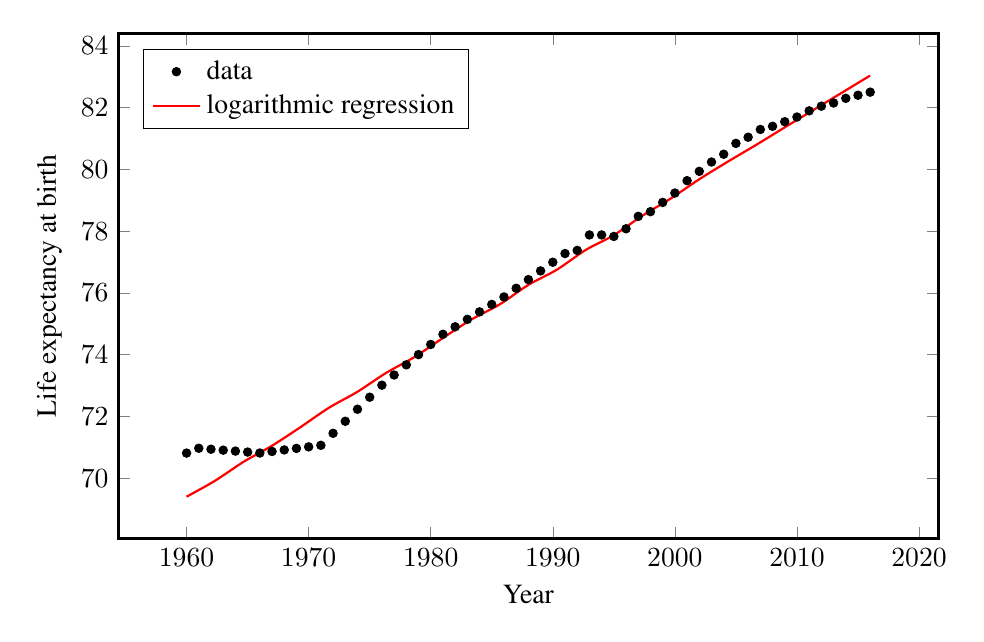
\begin{tikzpicture}
\tikzset{%%
  every mark/.append style={scale=1.0},%%
  scale=1.0%%
}
\pgfplotsset{%%
  every axis/.append style={font=\normalsize}%%
}
%%
\begin{axis}[%%
  axis line style=very thick,%%
  dotStyle/.style={mark size=1.5,black,mark color=black,mark=*,only marks},%%
  enlargelimits=true,%%
  height=8cm,%%
  legend cell align=left,%%
  legend pos=north west,%%
  plotStyle/.style={%%
    domain=1960:2016,%%
    mark=none,%%
    smooth,%%
    thick%%
  },%%
  width=12cm,%%
  %% x axis
  xlabel={\normalsize Year},%%
  xtick={1960,1970,1980,1990,2000,2010,2020},%%
  xticklabels={$1960$,$1970$,$1980$,$1990$,$2000$,$2010$,$2020$},%%
  %% y axis
  ylabel={\normalsize Life expectancy at birth}%%
]
%%
%%
\addplot[dotStyle] coordinates {
  (1960, 70.8170731707317)
  (1961, 70.9731707317073)
  (1962, 70.9424390243903)
  (1963, 70.9117073170732)
  (1964, 70.8809756097561)
  (1965, 70.850243902439)
  (1966, 70.819512195122)
  (1967, 70.8692682926829)
  (1968, 70.9190243902439)
  (1969, 70.9687804878049)
  (1970, 71.0185365853659)
  (1971, 71.0682926829268)
  (1972, 71.4575609756098)
  (1973, 71.8468292682927)
  (1974, 72.2360975609756)
  (1975, 72.6253658536586)
  (1976, 73.0146341463415)
  (1977, 73.3443902439024)
  (1978, 73.6741463414634)
  (1979, 74.0039024390244)
  (1980, 74.3336585365854)
  (1981, 74.6634146341463)
  (1982, 74.9048780487805)
  (1983, 75.1463414634146)
  (1984, 75.3878048780488)
  (1985, 75.6292682926829)
  (1986, 75.8707317073171)
  (1987, 76.1517073170732)
  (1988, 76.4326829268293)
  (1989, 76.7136585365854)
  (1990, 76.9946341463415)
  (1991, 77.2756097560976)
  (1992, 77.3780487804878)
  (1993, 77.8780487804878)
  (1994, 77.8780487804878)
  (1995, 77.8292682926829)
  (1996, 78.0780487804878)
  (1997, 78.4804878048781)
  (1998, 78.6317073170732)
  (1999, 78.9317073170732)
  (2000, 79.2341463414634)
  (2001, 79.6341463414634)
  (2002, 79.9365853658537)
  (2003, 80.2390243902439)
  (2004, 80.490243902439)
  (2005, 80.8414634146341)
  (2006, 81.0414634146342)
  (2007, 81.2926829268293)
  (2008, 81.3951219512195)
  (2009, 81.5439024390244)
  (2010, 81.6951219512195)
  (2011, 81.8951219512195)
  (2012, 82.0463414634146)
  (2013, 82.1487804878049)
  (2014, 82.3)
  (2015, 82.4)
  (2016, 82.5)
};
\addlegendentry{data}
%%
%%
\addplot+ [plotStyle,red]
{482.3980 * ln(x) - 3587.4517};
\addlegendentry{logarithmic regression}
\end{axis}
\end{tikzpicture}

\end{document}
